\documentclass[preview=true, border=10pt]{standalone}

\usepackage{tikz,pgfplots}
\pgfplotsset{compat=1.15}
\usetikzlibrary{calc,patterns,angles,quotes,arrows,arrows.meta}

\newcommand{\CKMTriangleTikzSize}{7.0}

\begin{document}
  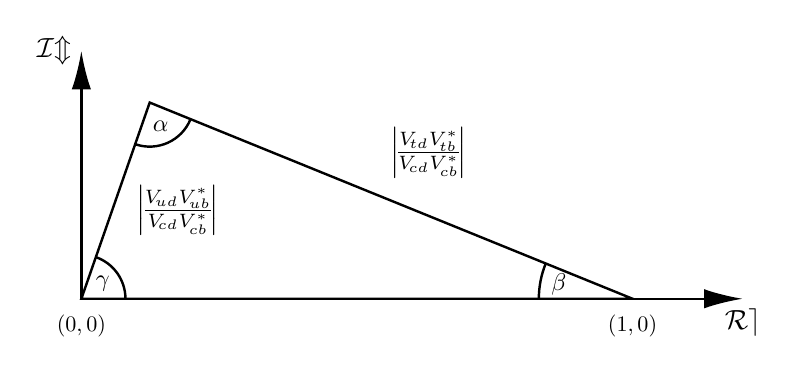
\begin{tikzpicture}[x=\CKMTriangleTikzSize cm, y=\CKMTriangleTikzSize cm, >=Latex]
    %draw coordinate system
    \draw [{Latex[width=\CKMTriangleTikzSize,length=2.0*\CKMTriangleTikzSize]}-{Latex[width=\CKMTriangleTikzSize,length=2.0*\CKMTriangleTikzSize]},
           line width = 0.125*\CKMTriangleTikzSize] (0,0.45) node (yaxis) [left, scale=1.0] {$\mathcal{I{}m}$}
                                                    |- (1.2,0) node (xaxis) [below, scale=1.0] {$\mathcal{R{}e}$};

    % draw triangle itself
    \draw[color=black, line width=0.125*\CKMTriangleTikzSize] (0.0,0.0) coordinate (g) -- (1.0,0.0) coordinate (b) -- (0.124,0.356) coordinate (a) -- cycle;

    % draw angles
    \pic[draw, -, pic text=$\beta$, line width=0.125*\CKMTriangleTikzSize,
         pic text options={scale=0.125*\CKMTriangleTikzSize},
         angle eccentricity=0.8, angle radius = 0.17*\CKMTriangleTikzSize cm]{angle = a--b--g};
    \pic[draw, -, pic text=$\alpha$, line width=0.125*\CKMTriangleTikzSize,
         pic text options={scale=0.125*\CKMTriangleTikzSize},
         angle eccentricity=0.6, angle radius = 0.08*\CKMTriangleTikzSize cm]{angle = g--a--b};
    \pic[draw, -, pic text=$\gamma$, line width=0.125*\CKMTriangleTikzSize,
         pic text options={scale=0.125*\CKMTriangleTikzSize},
         angle eccentricity=0.6, angle radius = 0.08*\CKMTriangleTikzSize cm]{angle = b--g--a};
    \node at(0.0, -0.05) [scale=0.8]{$(0,0)$};
    \node at(1.0, -0.05) [scale=0.8]{$(1,0)$};
    \node at(0.63, 0.265) [scale=1.0]{$\left|\!\frac{V_{{\kern -0.1em}td}V_{{\kern -0.1em}tb}^{*}}{V_{{\kern -0.1em}cd}V_{{\kern -0.1em}cb}^{*}}\!\right|$};
    \node at(0.175, 0.16) [scale=1.0]{$\left|\!\frac{V_{{\kern -0.1em}ud}V_{{\kern -0.1em}ub}^{*}}{V_{{\kern -0.1em}cd}V_{{\kern -0.1em}cb}^{*}}\!\right|$};
  \end{tikzpicture}
\end{document}
